\documentclass[a4paper,11pt]{article}
\usepackage{amsmath,amsthm,amsfonts,amssymb,amscd,amstext,vmargin,graphics,graphicx,tabularx,multicol} 
\usepackage[francais]{babel}
\usepackage[utf8]{inputenc}  
\usepackage[T1]{fontenc} 
\usepackage{pstricks-add,tikz,tkz-tab,variations}
\usepackage[autolanguage,np]{numprint} 

\setmarginsrb{1.5cm}{0.5cm}{1cm}{0.5cm}{0cm}{0cm}{0cm}{0cm} %Gauche, haut, droite, haut
\newcounter{numexo}
\newcommand{\exo}[1]{\stepcounter{numexo}\noindent{\bf \underline{Exercice~\thenumexo}}}
\reversemarginpar


\newcounter{enumtabi}
\newcounter{enumtaba}
\newcommand{\q}{\stepcounter{enumtabi} \theenumtabi.  }
\newcommand{\qa}{\stepcounter{enumtaba} (\alph{enumtaba}) }
\newcommand{\initq}{\setcounter{enumtabi}{0}}
\newcommand{\initqa}{\setcounter{enumtaba}{0}}

\newcommand{\be}{\begin{enumerate}}
\newcommand{\ee}{\end{enumerate}}
\newcommand{\bi}{\begin{itemize}}
\newcommand{\ei}{\end{itemize}}
\newcommand{\bp}{\begin{pspicture*}}
\newcommand{\ep}{\end{pspicture*}}
\newcommand{\bt}{\begin{tabular}}
\newcommand{\et}{\end{tabular}}
\renewcommand{\tabularxcolumn}[1]{>{\centering}m{#1}} %(colonne m{} centrée, au lieu de p par défault) 
\newcommand{\tnl}{\tabularnewline}

\newcommand{\bmul}[1]{\begin{multicols}{#1}}
\newcommand{\emul}{\end{multicols}}

\newcommand{\trait}{\noindent \rule{\linewidth}{0.2mm}}
\newcommand{\hs}[1]{\hspace{#1}}
\newcommand{\vs}[1]{\vspace{#1}}

\newcommand{\N}{\mathbb{N}}
\newcommand{\Z}{\mathbb{Z}}
\newcommand{\R}{\mathbb{R}}
\newcommand{\C}{\mathbb{C}}
\newcommand{\Dcal}{\mathcal{D}}
\newcommand{\Ccal}{\mathcal{C}}
\newcommand{\mc}{\mathcal}

\newcommand{\vect}[1]{\overrightarrow{#1}}
\newcommand{\ds}{\displaystyle}
\newcommand{\eq}{\quad \Leftrightarrow \quad}
\newcommand{\vecti}{\vec{\imath}}
\newcommand{\vectj}{\vec{\jmath}}
\newcommand{\Oij}{(O;\vec{\imath}, \vec{\jmath})}
\newcommand{\OIJ}{(O;I,J)}




\newcommand{\reponse}[1][1]{%
\multido{}{#1}{\makebox[\linewidth]{\rule[0pt]{0pt}{20pt}\dotfill}
}}

\newcommand{\titre}[5] 
% #1: titre #2: haut gauche #3: bas gauche #4: haut droite #5: bas droite
{
\noindent #2 \hfill #4 \\
#3 \hfill #5

\vspace{-1.6cm}

\begin{center}\rule{6cm}{0.5mm}\end{center}
\vspace{0.2cm}
\begin{center}{\large{\textbf{#1}}}\end{center}
\begin{center}\rule{6cm}{0.5mm}\end{center}
}



\begin{document}
\pagestyle{empty}
\titre{Chapitre 1 : Les nombres entiers}{}{}{}{}

\vspace*{1cm}

\begin{center}
{\Large \textbf{Niveau 1 :}}
\end{center}

\vspace*{1cm}

$\rightarrow$ \textbf{Écriture en chiffres}\\

\vspace*{0.5cm}

\exo \\

Écrire les nombres ci-dessous avec les bons espaces :\\

\bi
\item 2356 = . . . . . . . . . . . . . . . . . . . . .
\item 95430 = . . . . . . . . . . . . . . . . . . . . .
\item 1054896 = . . . . . . . . . . . . . . . . . . . . .\\
\ei


\exo \\

Choisir la réponse correcte parmi toutes celles proposées :\\

\begin{tabular}{|c|c|c|c|}
\hline 
25810 s'écrit : &  258 10 & 2 58 10 & 25 810 \\ 
\hline 
8654301 s'écrit : & 865 430 1 & 8 654 301 & 8 653 401 \\ 
\hline 
5257102013 s'écrit : & 5 257 102 013 & 52 571 213 & 525 710 201 3 \\ 
\hline 
\end{tabular} 
\vspace*{0.4cm}

\exo \\ Écrire les nombres suivants en chiffres :\\

\initqa
\qa cent treize  : . . . . . . . . . . . . . . . . . . . . . . . . . . . . . . . .\\

\qa cinq cent quatre-vingt huit : . . . . . . . . . . . . . . . . . . . . . . . . . . . . . . . . . . .\\

\qa quatre cent quatre-vingt quatre : . . . . . . . . . . . . . . . . . . . . . . . . . . . . . . . . . . .\\



 \exo \\ Écrire en chiffres les nombres soulignés dans les phrases.\\

\initqa \qa Burj Khalifa (Dubaï) est le plus haut des gratte-ciels, il culmine à \underline{huit cent vingt-huit} mètres : . . . . . . . . .\\

\qa Au Japon, le  mont Fuji culmine à \underline{trois mille sept cent soixante seize} mètres : . . . . . . . . .\\


\qa La distance de vol entre Marseille et Los Angeles est de \underline{neuf mille six cent quatre-vingt-dix-sept} kilomètres : . . . . . . . . .\\


\vspace*{0.6cm}



\vspace*{0.5cm}
$\rightarrow$  {\large \textbf{Écriture en lettres}}

\vspace*{0.5cm}


\exo \\ Écrire en lettres les nombres suivants :\\

\initqa \qa 13 = . . . . . . . . . . . . . . . . . . . . . . . . . . . . . . . . . . . . . . . . . . . . . . \\

\qa 28 = . . . . . . . . . . . . . . . . . . . . . . . . . . . . . . . . . . . . . . . . . . . . . . \\


\qa 52 = . . . . . . . . . . . . . . . . . . . . . . . . . . . . . . . . . . . . . . . . . . . . . . \\


\qa 74 = . . . . . . . . . . . . . . . . . . . . . . . . . . . . . . . . . . . . . . . . . . . . . . \\


\exo \\ Écrire en lettres les nombres suivants :\\

\initqa \qa 11 = . . . . . . . . . . . . . . . . . . . . . . . . . . . . . . . . . . . . . . . . . . . . . . \\

\qa 27 = . . . . . . . . . . . . . . . . . . . . . . . . . . . . . . . . . . . . . . . . . . . . . . \\


\qa 45 = . . . . . . . . . . . . . . . . . . . . . . . . . . . . . . . . . . . . . . . . . . . . . . \\


\qa 91 = . . . . . . . . . . . . . . . . . . . . . . . . . . . . . . . . . . . . . . . . . . . . . . \\





\vspace*{0.5cm}
$\rightarrow$  {\large \textbf{Zéros inutiles}}

\vspace*{0.5cm}


\exo \\ Réécrire les nombres suivants en supprimant les zéros inutiles si besoin.\\

\initqa \qa 100 = . . . . . . . . . . . . . . . . . . . . \\

\qa 010. . . . . . . . . . . . . . . . . . . . \\

\qa 002 = . . . . . . . . . . . . . . . . . . . . \\

\qa 0 020 = . . . . . . . . . . . . . . . . . . . . \\







\exo \\ Compléter par $=$ ou $\neq$.\\

\initqa \qa 34 . . . . . . . . . . 304\\

\qa 506 . . . . . . . . . . 056\\

\qa 0 900 . . . . . . . . . . 0 090\\

\qa 078 . . . . . . . . . . 78\\









\vspace*{0.5cm}
$\rightarrow$  {\large \textbf{Position des chiffres dans un nombre entier}}
\vspace*{0.5cm}




\exo\\ Compléter avec les mots : \textit{unités, dizaines, centaines, milliers, ...}\\

\initqa  \qa 327 = 3 . . . . . . . . . . 2 . . . . . . . . . . 7 . . . . . . . . . .\\

\qa 504 = 5 . . . . . . . . . . 4 . . . . . . . . . .\\


\qa 2 896 = 2 . . . . . . . . . . 8 . . . . . . . . . . 9 . . . . . . . . . . 6 . . . . . . . . . .\\





\exo \\ Dans 7 089 :\\

\initqa \qa le chiffre des unités est . . . .\\

\qa le chiffre des dizaines est  . . . .\\

\qa le chiffre des centaines est . . . .\\

\qa le chiffre des unités de mille est  . . . .\\


\exo \\ 70 532  spectateurs ont assisté à un match de football.\\

\initqa \qa 3 est le chiffre des . . . . . . . . . . . . . . . \\


\qa 0 est le chiffre des . . . . . . . . . . . . . . . \\

\qa 5 est le chiffre des . . . . . . . . . . . . . . . \\

\qa 2 est le chiffre des . . . . . . . . . . . . . . . \\



\vspace*{0.5cm}
$\rightarrow$  {\large \textbf{Décomposition d'un nombre entier}}
\vspace*{0.5cm}

\exo \\ Compléter les égalités suivantes.\\

\initqa \qa 1 235 = $ (1 \times . . . . . . . . . . .)+(2 \times . . . . . . . . . . . )+(3 \times . . . . . . . . . . .)+(5 \times . . . . . . . . . . .)$\\

\qa 9 418 = $ (. . . . . . . . . . . \times 1000)+(. . . . . . . . . . . \times 100 )+(. . . . . . . . . . . \times 10)+(. . . . . . . . . . . \times 1)$\\


\qa 24 106 = $ (2 \times . . . . . . . . . . .)+(4 \times . . . . . . . . . . . )+(1 \times . . . . . . . . . . .)+(6 \times . . . . . . . . . . .)$\\

\qa 758 014 = $ (7 \times . . . . . . . . . . .)+(5 \times . . . . . . . . . . . )+(8 \times . . . . . . . . . . .)+(1 \times . . . . . . . . . . .)+(4 \times . . . . . . . . . . .)$\\




\vspace*{0.5cm}
$\rightarrow$  {\large \textbf{Différentes écritures pour un même nombre entier}}
\vspace*{0.5cm}

\exo \\ Les nombres sur une même ligne sont tous identiques. Compléter les autres lignes comme sur le modèle de la première ligne.\\

\renewcommand{\arraystretch}{2}

\begin{tabular}{|c|c|c|}
\hline 
\hspace*{0.2cm} \textbf{En chiffres} \hspace*{0.2cm} & \hspace*{0.2cm} \textbf{En lettres} \hspace*{0.2cm} & \hspace*{0.2cm}\textbf{En décomposition} \hspace*{0.2cm} \\ 
\hline 
2 154 & Deux mille cent cinquante-quatre & $(2 \times 1000) + (1 \times 100) + (5 \times 10) + (4 \times 1)$ \\ 
\hline 
 &  & $(8 \times 1000) + (5 \times 100) +  (6 \times 1)$ \\ 
\hline 
 & Quinze mille treize &  \\ 
\hline 
\end{tabular} 






\vspace*{0.5cm}
$\rightarrow$  {\large \textbf{Différents systèmes de numération}}

\vspace*{0.5cm}



\exo \\ Écrire en chiffre romain  les nombres suivants :\\

\initqa \qa 14 = . . . . . . . . . . . . . \\

\qa 36 = . . . . . . . . . . . . . \\

\qa 52 = . . . . . . . . . . . . . \\

\qa 87 = . . . . . . . . . . . . . \\


\exo \\ Écrire en chiffre les nombres romains suivants :\\


\initqa \qa XVI = . . . . . . . . . . . . . \\

\qa XXXI = . . . . . . . . . . . . . \\

\qa LXIV = . . . . . . . . . . . . . \\

\qa XC = . . . . . . . . . . . . . \\


\vspace*{0.5cm}

\begin{center}
{\Large \textbf{Niveau 2 :}}
\end{center}

\vspace*{1cm}

$\rightarrow$ \textbf{Écriture en chiffres}\\

\vspace*{0.5cm}

\exo \\

Écrire les nombres ci-dessous avec les bons espaces :\\

\bi
\item 2563201 = . . . . . . . . . . . . . . . . . . . . .
\item 50026900 = . . . . . . . . . . . . . . . . . . . . .
\item 2598710543 = . . . . . . . . . . . . . . . . . . . . .\\
\ei


\exo \\

Choisir la réponse correcte parmi toutes celles proposées :\\

\begin{tabular}{|c|c|c|c|}
\hline 
9057412 s'écrit : &  905 741 2 & 9 05 74 12 & 9 057 412 \\ 
\hline 
10065820 s'écrit : & 100 658 20 & 10 065 820 & 10 056 820 \\ 
\hline 
6098087532 s'écrit : & 6 098 087 532  & 69 887 532 & 609 808 753 2 \\ 
\hline 
\end{tabular} 
\vspace*{0.4cm}

\exo \\ Écrire les nombres suivants en chiffres :\\

\initqa
\qa deux mille trois cent sept  : . . . . . . . . . . . . . . . . . . . . . . . . . . . . . . . .\\

\qa quatorze mille quatre-vingts : . . . . . . . . . . . . . . . . . . . . . . . . . . . . . . . . . . .\\

\qa dix-huit mille cent deux : . . . . . . . . . . . . . . . . . . . . . . . . . . . . . . . . . . .\\


 \exo \\ Écrire en chiffre les nombres soulignés dans les phrases.\\

\initqa \qa Le Chrysler Building est un gratte-ciel de la ville de New York, il culmine à environ \underline{deux cent quatre-vingt-deux} mètres : . . . . . . . . .\\

\qa Le mont Blanc, est le point culminant de la chaîne des Alpes avec une altitude de \underline{quatre mille huit cent neuf} mètres : . . . . . . . . .

\qa La distance de vol entre Paris et Bombay (en Inde) est de \underline{sept mille cinq } kilomètres: . . . . . . . . .\\




\vspace*{0.5cm}
$\rightarrow$  {\large \textbf{Écriture en lettres}}

\vspace*{0.5cm}


\exo \\ Écrire en lettres les nombres suivants :\\

\initqa \qa 932 = . . . . . . . . . . . . . . . . . . . . . . . . . . . . . . . . . . . . . . . . . . . . . . \\

\qa 671 = . . . . . . . . . . . . . . . . . . . . . . . . . . . . . . . . . . . . . . . . . . . . . . \\


\qa 3 804 = . . . . . . . . . . . . . . . . . . . . . . . . . . . . . . . . . . . . . . . . . . . . . . \\


\qa 1 507 = . . . . . . . . . . . . . . . . . . . . . . . . . . . . . . . . . . . . . . . . . . . . . . \\


\exo \\ Écrire en lettres les nombres suivants :\\

\initqa \qa 524 = . . . . . . . . . . . . . . . . . . . . . . . . . . . . . . . . . . . . . . . . . . . . . . \\

\qa 867 = . . . . . . . . . . . . . . . . . . . . . . . . . . . . . . . . . . . . . . . . . . . . . . \\


\qa 9 310 = . . . . . . . . . . . . . . . . . . . . . . . . . . . . . . . . . . . . . . . . . . . . . . \\


\qa 2 019 = . . . . . . . . . . . . . . . . . . . . . . . . . . . . . . . . . . . . . . . . . . . . . . \\



\vspace*{0.5cm}
$\rightarrow$  {\large \textbf{Zéros inutiles}}

\vspace*{0.5cm}


\exo \\ Réécrire les nombres suivants en supprimant les zéros inutiles si besoin.\\

\initqa \qa 0 303 = . . . . . . . . . . . . . . . . . . . . \\

\qa 3 030 = . . . . . . . . . . . . . . . . . . . . \\

\qa 4 000 = . . . . . . . . . . . . . . . . . . . . \\

\qa 04 004 = . . . . . . . . . . . . . . . . . . . . \\




\exo \\ Compléter par $=$ ou $\neq$.\\

\initqa \qa 12 . . . . . . . . . . 120\\

\qa 00580 . . . . . . . . . . 05800\\

\qa 004 . . . . . . . . . . 04\\

\qa 0608 . . . . . . . . . . 608\\



\vspace*{0.5cm}
$\rightarrow$  {\large \textbf{Position des chiffres dans un nombre entier}}
\vspace*{0.5cm}




\exo\\ Compléter avec les mots : \textit{unités, dizaines, centaines, milliers, ...}\\

\initqa  \qa 2 320 = 2 . . . . . . . . . . . . 3 . . . . . . . . . . . . 2 . . . . . . . . . . . . \\

\qa 4 630 091 = 4 . . . . . . . . . . . . 6 . . . . . . . . . . . . 3 . . . . . . . . . . . . 9 . . . . . . . . . . . . 1 . . . . . . . . . . . .\\

\qa 2 005 087 = 2 . . . . . . . . . . . . 5 . . . . . . . . . . . . 8 . . . . . . . . . . . . 7 . . . . . . . . . . . .\\







\exo \\ Dans 14 983 :\\

\initqa \qa le chiffre des centaines est . . . .\\

\qa le chiffre des unités de mille est  . . . .\\

\qa le chiffre des dizaines est . . . .\\

\qa le chiffre des unités est  . . . .\\


\exo \\ 180 597  spectateurs ont assisté à un match de rugby.\\

\initqa \qa 5 est le chiffre des . . . . . . . . . . . . . . . \\


\qa 8 est le chiffre des . . . . . . . . . . . . . . . \\

\qa 7 est le chiffre des . . . . . . . . . . . . . . . \\

\qa 0 est le chiffre des . . . . . . . . . . . . . . . \\


\exo \\  Compléter par les nombres qui conviennent.\\

\initqa \qa 1 milliard = . . . . . . . . millions\\

\qa 1 milliard = . . . . . . . . milliers\\

\qa 1 million = . . . . . . . . centaines\\

\qa 1 millier = . . . . . . . . dizaines\\


\vspace*{0.5cm}
$\rightarrow$  {\large \textbf{Décomposition d'un nombre entier}}
\vspace*{0.5cm}

\exo \\ Compléter les égalités avec le nombre entier correspondant ou sa décomposition.\\

\initqa \qa 7 480 = . . . . . . . . . . . . . . . . . . . . . . . . . . . . . . . . . . . . . . . . . . . . . . . . . . . . . . . . . . . .\\

\qa . . . . . . . . . . . . . . . = $ (2 \times 10 000 )+(8 \times 1 000)+(1 \times 100)+(4 \times 10) + (5 \times 1)$


\qa  347 618 = . . . . . . . . . . . . . . . . . . . . . . . . . . . . . . . . . . . . . . . . . . . . . . . . . . . . . . . . . . . .\\

\qa . . . . . . . . . . . . . . . = $ (8 \times 1 000 000)+(5 \times 100 000)+(3 \times 10 000 )+(6 \times 100)+(7 \times 10) + (5 \times 1)$\\

\vspace*{0.5cm}
$\rightarrow$  {\large \textbf{Différentes écritures pour un même nombre entier}}
\vspace*{0.5cm}

\exo \\ Les nombres sur une même ligne sont tous identiques. Compléter les autres lignes comme sur le modèle de la première ligne.\\

\renewcommand{\arraystretch}{2}

\begin{tabular}{|p{3cm}|p{4cm}|p{9cm}|}
\hline 
\hspace*{0.2cm} \textbf{En chiffres} \hspace*{0.2cm} & \hspace*{0.2cm} \textbf{En lettres} \hspace*{0.2cm} & \hspace*{0.2cm}\textbf{En décomposition} \hspace*{0.2cm} \\ 
\hline 
2 154 & Deux mille cent cinquante-quatre & $(2 \times 1000) + (1 \times 100) + (5 \times 10) + (4 \times 1)$ \\ 
\hline 
106 980 &  &  \\ 
\hline 
 & Cinq cent six mille trois cent cinquante huit   &  \\ 
\hline 
 &  & $(9 \times 100 000 ) + (2 \times  1 000) + ( 6 \times 100 ) + (1 \times 10 ) + (8 \times 1)$ \\ 
\hline 
\end{tabular} 

\vspace*{0.5cm}
$\rightarrow$  {\large \textbf{Différents systèmes de numération}}

\vspace*{0.5cm}



\exo \\ Écrire en chiffre romain  les nombres suivants :\\

\initqa \qa 127 = . . . . . . . . . . . . . \\

\qa 412 = . . . . . . . . . . . . . \\

\qa 500 = . . . . . . . . . . . . . \\

\qa 739 = . . . . . . . . . . . . . \\


\exo \\ Écrire en chiffre les nombres romains suivants :\\


\initqa \qa DIX = . . . . . . . . . . . . . \\

\qa CDLXXIII = . . . . . . . . . . . . . \\

\qa DCXXI = . . . . . . . . . . . . . \\

\qa CMXI = . . . . . . . . . . . . . \\


\vspace*{0.5cm}



\begin{center}
{\Large \textbf{Niveau 3 :}}
\end{center}

\vspace*{1cm}

$\rightarrow$ \textbf{Écriture en chiffres}\\

\vspace*{0.5cm}

\exo \\

Écrire les nombres ci-dessous avec les bons espaces :\\

\bi
\item 80652014 = . . . . . . . . . . . . . . . . . . . . .
\item 100584712 = . . . . . . . . . . . . . . . . . . . . .
\item 38790125047 = . . . . . . . . . . . . . . . . . . . . .\\
\ei


\exo \\

Choisir la réponse correcte parmi toutes celles proposées :\\

\begin{tabular}{|c|c|c|c|}
\hline 
50239417 s'écrit : &  502 394 17 & 5 02 39 41 7 & 50 239 417\\ 
\hline 
6930047801 s'écrit : & 693 004 780 1 & 6 930 047 801 & 6 930 407 801 \\ 
\hline 
52874196800 s'écrit : & 52 874 796 800  & 528 741 968 & 528 741 968 000 \\ 
\hline 
\end{tabular} 
\vspace*{0.4cm}

\exo \\ Écrire les nombres suivants en chiffres :\\

\initqa
\qa sept cent trente-quatre mille huit cents  : . . . . . . . . . . . . . . . . . . . . . . . . . . . . . . . .\\

\qa trois millions neuf cent quatre-vingt-trois mille cinq cent cinquante et un  : . . . . . . . . . . . . . . . . . . . . . . . . . . . . . . . . . . .\\

\qa vingt millions quinze mille cent quarante-six    : . . . . . . . . . . . . . . . . . . . . . . . . . . . . . . . . . . .\\

\exo \\ Écrire en chiffre les nombres soulignés dans les phrases.\\

\initqa \qa La tour Eiffel est une tour de fer pesant plus de \underline{ dix mille cents} tonnes : . . . . . . . . .\\

\qa Le rayon de la Terre, c'est-à-dire la distance entre le centre de la Terre et sa surface, est d'environ \underline{six mille trois cent soixante et onze} km  : . . . . . . . . .\\


\qa La distance de la Terre à la Lune est d'environ \underline{trois cent quatre-vingt-quatre mille quatre cents} kilomètres : . . . . . . . . .\\

\vspace*{0.5cm}
$\rightarrow$  {\large \textbf{Écriture en lettres}}

\vspace*{0.5cm}


\exo \\ Écrire en lettres les nombres suivants :\\

\initqa \qa 120 = . . . . . . . . . . . . . . . . . . . . . . . . . . . . . . . . . . . . . . . . . . . . . . \\

\qa 900 = . . . . . . . . . . . . . . . . . . . . . . . . . . . . . . . . . . . . . . . . . . . . . . \\


\qa 1 527 = . . . . . . . . . . . . . . . . . . . . . . . . . . . . . . . . . . . . . . . . . . . . . . \\


\qa 6 480 = . . . . . . . . . . . . . . . . . . . . . . . . . . . . . . . . . . . . . . . . . . . . . . \\


\exo \\ Écrire en lettres les nombres suivants :\\

\initqa \qa 380 = . . . . . . . . . . . . . . . . . . . . . . . . . . . . . . . . . . . . . . . . . . . . . . \\

\qa 1 187 = . . . . . . . . . . . . . . . . . . . . . . . . . . . . . . . . . . . . . . . . . . . . . . \\


\qa 5 100 = . . . . . . . . . . . . . . . . . . . . . . . . . . . . . . . . . . . . . . . . . . . . . . \\


\qa 10 426 = . . . . . . . . . . . . . . . . . . . . . . . . . . . . . . . . . . . . . . . . . . . . . . \\

\vspace*{0.5cm}
$\rightarrow$  {\large \textbf{Zéros inutiles}}

\vspace*{0.5cm}


\exo \\ Réécrire les nombres suivants en supprimant les zéros inutiles si besoin.\\

\initqa \qa 008 050 = . . . . . . . . . . . . . . . . . . . . \\

\qa 005 505 = . . . . . . . . . . . . . . . . . . . . \\

\qa 055 005 = . . . . . . . . . . . . . . . . . . . . \\

\qa 666 000 = . . . . . . . . . . . . . . . . . . . . \\

\qa 006 606 = . . . . . . . . . . . . . . . . . . . . \\



\exo \\ Compléter par $=$ ou $\neq$.\\

\initqa \qa 00540 . . . . . . . . . . 0504\\

\qa 06005 . . . . . . . . . . 6005\\

\qa 070080 . . . . . . . . . . 700800\\

\qa 004750 . . . . . . . . . . 4750\\

\qa 010005800 . . . . . . . . . . . . 100005800\\



\vspace*{0.5cm}
$\rightarrow$  {\large \textbf{Position des chiffres dans un nombre entier}}
\vspace*{0.5cm}




\exo \\ Dans le nombre 56 940 238 :\\

\initqa

\qa le chiffre des dizaines de mille est  . . . .\\

\qa  le chiffre des centaines est  . . . .\\

\qa le chiffre des unités de millions est . . . .\\

\qa le chiffre de dizaines est  . . . .\\




\exo \\ Compléter par les nombres qui conviennent.\\

\initqa \qa Quatre dizaines, c'est . . . . . . . unités.\\

\qa Six centaines, c'est . . . . . . . unités.\\

\qa Trois milliers, c'est . . . . . . . unités.\\

\qa Neuf milliards, c'est . . . . . . . unités.\\

\exo \\ Donner l'écriture en chiffres des nombres suivants.\\

\initqa \qa 7 dizaines = . . . . . . . . . . . . . . . . . .\\

\qa 25 dizaines = . . . . . . . . . . . . . . . . . .\\


\qa 8 centaines = . . . . . . . . . . . . . . . . . .\\


\qa 68 centaines = . . . . . . . . . . . . . . . . . .\\


\vspace*{0.5cm}
$\rightarrow$  {\large \textbf{Décomposition d'un nombre entier}}
\vspace*{0.5cm}

\exo \\ Compléter les égalités avec le nombre entier correspondant ou sa décomposition.\\

\initqa \qa 7 108 620= . . . . . . . . . . . . . . . . . . . . . . . . . . . . . . . . . . . . . . . . . . . . . . . . . . . . . . . . . . . .\\

\qa . . . . . . . . . . . . . . . = $ (1 \times 10 000 000 )+(5 \times 1 000 000)+(7 \times 10)+(3 \times 1) $\\


\qa  651 000 000 = . . . . . . . . . . . . . . . . . . . . . . . . . . . . . . . . . . . . . . . . . . . . . . . . . . . . . . . . . . . .\\

\qa . . . . . . . . . . . . . . . = $ (9 \times 100 000 000)+(8 \times 10 000 000)+(5 \times 100 000 )+(4 \times 1 000)+(1 \times 100) + (7 \times 10)$\\


\vspace*{0.5cm}
$\rightarrow$  {\large \textbf{Différentes écritures pour un même nombre entier}}
\vspace*{0.5cm}

\exo \\ Les nombres sur une même ligne sont tous identiques. Compléter les autres lignes comme sur le modèle de la première ligne.\\

\renewcommand{\arraystretch}{2}

\begin{tabular}{|p{3cm}|p{4cm}|p{9cm}|}
\hline 
\hspace*{0.2cm} \textbf{En chiffres} \hspace*{0.2cm} & \hspace*{0.2cm} \textbf{En lettres} \hspace*{0.2cm} & \hspace*{0.2cm}\textbf{En décomposition} \hspace*{0.2cm} \\ 
\hline 
2 154 & Deux mille cent cinquante-quatre & $(2 \times 1 000) + (1 \times 100) + (5 \times 10) + (4 \times 1)$ \\ 
\hline 
 & Neuf millions huit cent quatre-vingt-dix-huit mille deux cent six &  \\ 
\hline 
 &   & $ (3 \times 1 000 000 )+( 4 \times 100 000)+(9 \times 10 000)+(8 \times 1 000) + (5 \times 100) +(2 \times 1)$ \\ 
\hline 
120 456 827 &  &  \\ 
\hline 
\end{tabular} 


\vspace*{0.5cm}
$\rightarrow$  {\large \textbf{Différents systèmes de numération}}

\vspace*{0.5cm}



\exo \\ Écrire en chiffre romain  les nombres suivants :\\

\initqa \qa 666 = . . . . . . . . . . . . . \\

\qa 1 492 = . . . . . . . . . . . . . \\

\qa 1 999 = . . . . . . . . . . . . . \\

\qa 2 019 = . . . . . . . . . . . . . \\


\exo \\ Écrire en chiffre les nombres romains suivants :\\


\initqa \qa MMDCCLXVI = . . . . . . . . . . . . . \\

\qa MCMLXXXIV = . . . . . . . . . . . . . \\

\qa MDCXXXVII = . . . . . . . . . . . . . \\

\qa MDCCLXIX = . . . . . . . . . . . . . \\





\vspace*{0.5cm}

\begin{center}
{\Large \textbf{Niveau 4:}}
\end{center}

\vspace*{1cm}

$\rightarrow$ \textbf{Écriture en chiffres}\\

\vspace*{0.5cm}


\exo \\

Écrire les nombres ci-dessous avec les bons espaces :\\

\bi
\item 789067 = . . . . . . . . . . . . . . . . . . . . .
\item 80932576943 = . . . . . . . . . . . . . . . . . . . . .
\item 63107005 = . . . . . . . . . . . . . . . . . . . . .
\item 5012000721 = . . . . . . . . . . . . . . . . . . . . .\\
\ei


\exo \\

Choisir la réponse correcte parmi toutes celles proposées :\\

\begin{tabular}{|c|c|c|c|}
\hline 
95432187621 s'écrit : &  954 321 876 21 & 95 43 21 87 62 1 & 95 432 187 621\\ 
\hline 
3570095128642 s'écrit : & 357 951 286 42 & 3 570 095 128 642 & 357 095 128 642 \\ 
\hline 
12500369421450 s'écrit : & 12 500 369 421 450  & 125 369 421 450 & 1 250 036 942 145 \\ 
\hline 
\end{tabular} 
\vspace*{0.4cm}

\exo \\ Écrire les nombres suivants en chiffres :\\

\initqa
\qa soixante-dix mille neuf cent sept  : . . . . . . . . . . . . . . . . . . . . . . . . . . . . . . . .\\

\qa Cinq millions cinq cent douze mille : . . . . . . . . . . . . . . . . . . . . . . . . . . . . . . . . . . .\\

\qa Huit milliards sept cent millions    : . . . . . . . . . . . . . . . . . . . . . . . . . . . . . . . . . . .\\

\exo \\ Écrire en chiffres les nombres soulignés dans les phrases.\\

\initqa \qa L'Everest est le plus haut sommet du globe, avec un pic à \underline{huit mille huit cent quarante-huit} mètres d'altitude.: . . . . . . . . .\\

\qa La distance de la Terre au soleil est d'environ \underline{cent quarante neuf millions cinq cent quatre-vingt-dix-sept mille huit cent soixante-dix}  : . . . . . . . . .\\


\qa La population mondiale est estimée à \underline{sept milliards cinq cent cinquante millions soixante-quatorze} au 1er juillet 2017  : . . . . . . . . .\\


\vspace*{0.5cm}
$\rightarrow$  {\large \textbf{Écriture en lettres}}

\vspace*{0.5cm}


\exo \\ Écrire en lettres les nombres suivants :\\

\initqa \qa 156 320 = . . . . . . . . . . . . . . . . . . . . . . . . . . . . . . . . . . . . . . . . . . . . . . \\

\qa 77 208 = . . . . . . . . . . . . . . . . . . . . . . . . . . . . . . . . . . . . . . . . . . . . . . \\


\qa 1 394 299 = . . . . . . . . . . . . . . . . . . . . . . . . . . . . . . . . . . . . . . . . . . . . . . \\


\qa 20 579 081 = . . . . . . . . . . . . . . . . . . . . . . . . . . . . . . . . . . . . . . . . . . . . . . \\


\exo \\ Écrire en lettres les nombres suivants :\\

\initqa \qa 84 123 = . . . . . . . . . . . . . . . . . . . . . . . . . . . . . . . . . . . . . . . . . . . . . . \\

\qa 741 300 = . . . . . . . . . . . . . . . . . . . . . . . . . . . . . . . . . . . . . . . . . . . . . . \\


\qa 4 630 041 = . . . . . . . . . . . . . . . . . . . . . . . . . . . . . . . . . . . . . . . . . . . . . . \\


\qa 57 195 000 = . . . . . . . . . . . . . . . . . . . . . . . . . . . . . . . . . . . . . . . . . . . . . . \\

\exo \\ Compléter le texte ci-dessous en écrivant cette fois chaque nombre en toutes lettres.\\

La   région  Ile-de-France   est   une   région   française   qui regroupe \textbf{8} départements. \\
Elle a une superficie d'environ \textbf{12 000} $km^{2}$ et une population de \textbf{13 082 144} habitants.\\
Paris possède environ \textbf{2 206 400} habitants en comparaison Malakoff en possède \textbf{30 225}.\\

\vspace*{0.4cm}

La   région  Ile-de-France   est   une   région   française   qui regroupe . . . . . . . . . . . . . . . . . . . . . . . . . . départements. \\
Elle a une superficie d'environ . . . . . . . . . . . . . . . . . . . . . . . . . . et une population de . . . . . . . . . . . . . . . . . . . . . . . . . . habitants.\\
Paris possède environ . . . . . . . . . . . . . . . . . . . . . . . . . . habitants en comparaison Malakoff en possède . . . . . . . . . . . . . . . . . . . . . . . . . . .\\

\vspace*{0.5cm}
$\rightarrow$  {\large \textbf{Zéros inutiles}}

\vspace*{0.5cm}


\exo \\ Réécrire les nombres suivants en supprimant les zéros inutiles si besoin.\\

\initqa \qa 007 800 = . . . . . . . . . . . . . . . . . . . . \\

\qa 06 010 010 = . . . . . . . . . . . . . . . . . . . . \\

\qa 050 009 320 = . . . . . . . . . . . . . . . . . . . . \\

\qa 600 000 000 = . . . . . . . . . . . . . . . . . . . . \\

\qa 000 808 400 = . . . . . . . . . . . . . . . . . . . . \\



\exo \\ Compléter par $=$ ou $\neq$.\\

\initqa \qa  041410 . . . . . . . . . . 00414100\\

\qa 7070700 . . . . . . . . . . 007070700\\

\qa 029610090 . . . . . . . . . . 00296100090\\

\qa  00600003 . . . . . . . . . . 06000300\\

\qa  0050008000. . . . . . . . . . . . 00500800\\



\vspace*{0.5cm}
$\rightarrow$  {\large \textbf{Position des chiffres dans un nombre entier}}
\vspace*{0.5cm}




\exo \\ Dans le nombre 98 651 :\\

\initqa

\qa le chiffre des centaines est  . . . .\\

\qa  le nombre de centaines est  . . . .\\

\qa le chiffre des unités est . . . .\\

\qa le nombre d'unités est  . . . .\\




\exo \\ Compléter par les nombres qui conviennent.\\

\initqa \qa Dix dizaines, c'est . . . . . . . unités.\\

\qa Cinq centaines, c'est . . . . . . . dizaines.\\

\qa Deux milliers, c'est . . . . . . . dizaines.\\

\qa Neuf millions, c'est . . . . . . . centaines.\\


\exo \\ Donner l'écriture en chiffres des nombres suivants.\\

\initqa \qa 370 dizaines = . . . . . . . . . . . . . . . . . .\\

\qa 25 centaines = . . . . . . . . . . . . . . . . . .\\

\qa 325 centaines = . . . . . . . . . . . . . . . . . .\\

\qa 40 dizaines de milliers = . . . . . . . . . . . . . . . . . .\\

\exo \\
Je suis un nombre entier. \\
-  Mon nombre de dizaines de milliers est 5 406.  \\
-  Mon chiffre des centaines est la moitié de mon chiffre des unités de millions. \\
-  Mon chiffre des unités de milliers est le même que celui du nombre 49 230. \\
-  Mon chiffre des unités est égal à la différence de mon chiffre des unités de milliers et de mon chiffre des centaines. \\
-  Mon chiffre des dizaines est égal à la somme de mon chiffre des centaines et de mon chiffre des unités. \\
  Qui suis-je ? \\



\vspace*{0.5cm}
$\rightarrow$  {\large \textbf{Différentes écritures pour un même nombre entier}}
\vspace*{0.5cm}

\exo \\ Les nombres sur une même ligne sont tous identiques. Compléter les autres lignes comme sur le modèle de la première ligne.\\

\renewcommand{\arraystretch}{2}

\begin{tabular}{|p{3cm}|p{4cm}|p{9cm}|}
\hline 
\hspace*{0.2cm} \textbf{En chiffres} \hspace*{0.2cm} & \hspace*{0.2cm} \textbf{En lettres} \hspace*{0.2cm} & \hspace*{0.2cm}\textbf{En décomposition} \hspace*{0.2cm} \\ 
\hline 
2 154 & Deux mille cent cinquante-quatre & $(2 \times 1 000) + (1 \times 100) + (5 \times 10) + (4 \times 1)$ \\ 
\hline 
  & Dix milliards trois cent quatorze millions sept cent vingt mille soixante-dix-neuf &   \\ 
\hline 
3 404 150 680 &   & \\ 
\hline 
 &  & $(5 \times 1 000 000 000) + (4 \times 100 000 000 ) +(9 \times 10 000 000 ) +(2 \times 100 000) +(8 \times 10 000)+(1 \times 100) + (3 \times 10)$  \\ 
\hline 
\end{tabular} 


\vspace*{0.5cm}
$\rightarrow$  {\large \textbf{Décomposition d'un nombre entier}}
\vspace*{0.5cm}

\exo \\ Compléter les égalités avec le nombre entier correspondant ou sa décomposition.\\

\initqa \qa 879 120 000= . . . . . . . . . . . . . . . . . . . . . . . . . . . . . . . . . . . . . . . . . . . . . . . . . . . . . . . . . . . .\\

\qa . . . . . . . . . . . . . . . = $ (8 \times 1 000 000 000 )+(1 \times 100 000 000) $\\


\qa  172 500 000 000 = . . . . . . . . . . . . . . . . . . . . . . . . . . . . . . . . . . . . . . . . . . . . . . . . . . . . . . . . . . . .\\



\qa . . . . . . . . . . . . . . . = $ (3 \times 1 000 000 000)+(5 \times 100  000 000)+(5 \times 1 000 000 )+(1 \times 10 000)$\\


\vspace*{0.5cm}
$\rightarrow$  {\large \textbf{Différents systèmes de numération}}

\vspace*{0.5cm}
 
\exo \\ Dans la numération égyptienne, chaque ordre de grandeur possède un symbole qui qu'il faut répéter le nombre de fois nécessaire.\\

\includegraphics[scale=0.8]{numerationegyptienne1.eps} \\

Quels sont les nombres suivants ?\\


\includegraphics[scale=0.9]{numerationegyptienne2.eps} = . . . . . . . . . 
\includegraphics[scale=0.9]{numerationegyptienne3.eps} = . . . . . . . . . 
\includegraphics[scale=0.9]{numerationegyptienne4.eps} = . . . . . . . . .\\


\exo \\ Dans la numération égyptienne, chaque ordre de grandeur possède un symbole qui qu'il faut répéter le nombre de fois nécessaire.\\

\includegraphics[scale=0.8]{numerationegyptienne1.eps} \\

Quels sont les nombres suivants ?\\


\includegraphics[scale=0.9]{numerationegyptienne5.eps} = . . . . . . . . . 
\includegraphics[scale=0.9]{numerationegyptienne6.eps} = . . . . . . . . . 
\includegraphics[scale=0.9]{numerationegyptienne7.eps} = . . . . . . . . .\\



\begin{center}
{\Large \textbf{Niveau 5 :}}
\end{center}

\vspace*{1cm}

$\rightarrow$ \textbf{Écriture en chiffres}\\

\vspace*{0.5cm}

\exo \\

Écrire les nombres ci-dessous avec les bons espaces :\\

\bi
\item 25478921 = . . . . . . . . . . . . . . . . . . . . .
\item 2530014897010 = . . . . . . . . . . . . . . . . . . . . .
\item 2648951370000 = . . . . . . . . . . . . . . . . . . . . .
\item 20350680017890 = . . . . . . . . . . . . . . . . . . . . .\\
\ei


\exo \\

Choisir la réponse correcte parmi toutes celles proposées :\\

\begin{tabular}{|c|c|c|c|}
\hline 
320158094627 s'écrit : &  320 158 094 627 & 32 01 58 0946 27 & 32 158 094 627\\ 
\hline 
5698710254090 s'écrit : & 569 871 025 409 0 & 5 698 710 254 090 & 569 871 025 409 \\ 
\hline 
50036487941000 s'écrit : & 536 487 941 000  & 50 036 487 941 & 50 036 487 941 000 \\ 
\hline 
\end{tabular} 
\vspace*{0.4cm}

\exo \\ Écrire les nombres suivants en chiffres :\\

\initqa
\qa neuf cent soixante-dix-sept mille deux  : . . . . . . . . . . . . . . . . . . . . . . . . . . . . . . . .\\

\qa Quatre cent millions cinquante mille vingts : . . . . . . . . . . . . . . . . . . . . . . . . . . . . . . . . . . .\\

\qa Dix milliards seize mille    : . . . . . . . . . . . . . . . . . . . . . . . . . . . . . . . . . . .\\

\exo \\ Écrire en chiffre les nombres soulignés dans les phrases.\\

\initqa \qa Il y a \underline{trois mille six cents} secondes dans une heure . . . . . . . . .\\

\qa L'âge de la Terre est, selon les connaissances actuelles, de \underline{quatre milliards} d'années  : . . . . . . . . .\\


\qa Les requins sont sur Terre depuis plus de \underline{quatre cent cinquante millions } d'années : . . . . . . . . .\\

\vspace*{0.5cm}
$\rightarrow$  {\large \textbf{Écriture en lettres}}

\vspace*{0.5cm}


\exo \\ Écrire en lettres les nombres suivants :\\

\initqa \qa 100 324 765 = . . . . . . . . . . . . . . . . . . . . . . . . . . . . . . . . . . . . . . . . . . . . . . \\

\qa 1 000 354 111 = . . . . . . . . . . . . . . . . . . . . . . . . . . . . . . . . . . . . . . . . . . . . . . \\


\qa 7 003 500 471 = . . . . . . . . . . . . . . . . . . . . . . . . . . . . . . . . . . . . . . . . . . . . . . \\


\qa 18 040 009 706 = . . . . . . . . . . . . . . . . . . . . . . . . . . . . . . . . . . . . . . . . . . . . . . \\


\exo \\ Écrire en lettres les nombres suivants :\\

\initqa \qa 1 000 427 = . . . . . . . . . . . . . . . . . . . . . . . . . . . . . . . . . . . . . . . . . . . . . . \\

\qa 19 000 500 080 = . . . . . . . . . . . . . . . . . . . . . . . . . . . . . . . . . . . . . . . . . . . . . . \\


\qa 301 402 000 026 = . . . . . . . . . . . . . . . . . . . . . . . . . . . . . . . . . . . . . . . . . . . . . . \\


\qa 3 000 000 069 = . . . . . . . . . . . . . . . . . . . . . . . . . . . . . . . . . . . . . . . . . . . . . . \\


\exo \\ Compléter le texte ci-dessous en écrivant cette fois chaque nombre en toutes lettres.\\

L'Europe est un continent composé de \textbf{50} pays différents où vivent \textbf{743 000 000} personnes sur une superficie de \textbf{10 180 000} $km^{2}$.\\
En comparaison, l'Asie composée de \textbf{50} pays différents également a une superficie de \textbf{43 810 582} $km^{2}$ pour \textbf{4 342 255 000} habitants.\\

\vspace*{0.4cm}

 L'Europe est un continent composé de . . . . . . . . . . . . . . . . . . . . . . . . pays différents où vivent . . . . . . . . . . . . . . . . . . . . . . . . personnes sur une superficie de . . . . . . . . . . . . . . . . . . . . . . . . $km^{2}$.\\
En comparaison, l'Asie composée de . . . . . . . . . . . . . . . . . . . . . . . . pays différents également a une superficie de . . . . . . . . . . . . . . . . . . . . . . . . $km^{2}$ pour . . . . . . . . . . . . . . . . . . . . . . . . habitants.\\

\vspace*{0.5cm}
$\rightarrow$  {\large \textbf{Zéros inutiles}}

\vspace*{0.5cm}


\exo \\ Réécrire les nombres suivants en supprimant les zéros inutiles si besoin.\\

\initqa \qa 005 001 000 = . . . . . . . . . . . . . . . . . . . . \\

\qa 074 013 0690 = . . . . . . . . . . . . . . . . . . . . \\

\qa 800 009 000  = . . . . . . . . . . . . . . . . . . . . \\

\qa 03 007 400 010 = . . . . . . . . . . . . . . . . . . . . \\

\qa 706 001 000 200 = . . . . . . . . . . . . . . . . . . . . \\



\exo \\ Compléter par $=$ ou $\neq$.\\

\initqa \qa 0002030500  . . . . . . . . . . 20305\\

\qa  00016500870 . . . . . . . . . . 16500780 \\

\qa 040000090 . . . . . . . . . . 0004000090\\

\qa 000700005000  . . . . . . . . . . 700005000 \\

\qa 08010065200  . . . . . . . . . . . . 80100652\\

\exo \\ Écrire tous les nombres entiers possibles de trois chiffres en utilisant une seule fois chacun des chiffres 3 ; 4 et 0.\\
\reponse[3]

\exo \\ Le 28 septembre 2015 (28 09 2015) s'écrit avec seulement avec 6 chiffres différents : 2 , 8 , 0 , 9 , 1 et 5. \\
Quelle a été la dernière date à s'écrire à l'aide de 8 chiffres  tous différents ? \\
\reponse[2]


\vspace*{0.5cm}
$\rightarrow$  {\large \textbf{Position des chiffres dans un nombre entier}}
\vspace*{0.5cm}




\exo \\ Dans le nombre 7 156 940 238 :\\
\initqa

\qa  le chiffre des unités de milliards est  . . . . . . . . . . . .\\

\qa  le nombre d'unités de millions est . . . . . . . . . . . . \\

\qa le chiffre des dizaines  de mille est . . . . . . . . . . . .\\

\qa le nombre de centaines est  . . . . . . . . . . . . \\




\exo \\ Donner l'écriture en chiffres des nombres suivants.\\

\initqa \qa 7 654 dizaines = . . . . . . . . . . . . . . . . . .\\

\qa 21 dizaines de mille et 87 unités = . . . . . . . . . . . . . . . . . .\\


\qa 150 unités de millions = . . . . . . . . . . . . . . . . . .\\


\qa 69 unités de millions et 146 dizaines = . . . . . . . . . . . . . . . . . .\\


\exo\\ Ajouter des zéros (s'il en faut) pour que 5 soit le chiffre \textit{des dizaines de mille} de chaque nombre :\\

9785	\hspace*{3cm}		7503		\hspace*{3cm}		251039	\hspace*{3cm}			1256\\








\vspace*{5cm}

\exo \\ Compléter les égalités avec le nombre correspondant ou sa décomposition.\\

20 154 = . . . . . . . . . . . . . . . . . . . . . . . . . . . . . . . . . . . . . . . . . . . . . . . . . . . . . . . . . . . . \\

. . . . . . . . . . . . . . . . . . . . . . =  (8 $\times$ 1 000) + ( 5 $\times$ 100) + 6\\

8 000  907 = . . . . . . . . . . . . . . . . . . . . . . . . . . . . . . . . . . . . . . . . . . . . . . . . . . . . . . . . . . . . \\

. . . . . . . . . . . . . . . . . . . . . . . . . =  (3 $\times$ 1 000 000 000) + ( 2 $\times$ 10 000) + (4 $\times$ 1 000) + (8 $\times$ 10)\\

\vspace*{0.6cm}

\exo \\ Dans le nombre 7 156 940 238 :\\
\initqa

\qa  quel est le chiffre des unités de milliards ?  .....................\\

\qa  quel est le nombre d'unités de millions ?  .................. \\

\qa quel est le chiffre des centaines ? ..................\\

\qa quel est le nombre de dizaines ?  ................. \\


\exo\\

Je suis un nombre entier à onze chiffres. \\
-  Mon chiffre des unités est le double de 3. \\
-  Mon chiffre des centaines de mille est égal à la moitié de mon chiffre des unités. \\
-  Mon chiffre des dizaines de millions est égal au tiers de mon chiffre des unités. \\
-  La somme de mon chiffre des centaines de mille et de mon chiffre des centaines est égale à 8. \\
-  La différence entre mon chiffre des unités et mon chiffre des dizaines est égale à 5. \\
-  Le produit de mon chiffre des dizaines de millions par mon chiffre des dizaines de milliards est égal à la somme des trois chiffres de la classe des unités.  \\
-  La somme de mon chiffre des centaines et de mon chiffre des centaines de mille est égale à la somme de mon chiffre des dizaines et de mon chiffre des centaines de millions. \\
-  Mon chiffre des unités de millions est le quadruple de mon chiffre des dizaines de millions. \\
- Tous les chiffres sont présents au moins une fois dans mon écriture et mon chiffre des unités de mille est supérieur à mon chiffre des dizaines de mille, lui-même supérieur à mon chiffre des unités de milliards. \\
Qui suis-je?\\

\vspace*{0.5cm}
$\rightarrow$  {\large \textbf{Décomposition d'un nombre entier}}
\vspace*{0.5cm}

\exo \\ Compléter les égalités avec le nombre entier correspondant ou sa décomposition.\\

\initqa \qa 20 507 050= . . . . . . . . . . . . . . . . . . . . . . . . . . . . . . . . . . . . . . . . . . . . . . . . . . . . . . . . . . . .\\

\qa . . . . . . . . . . . . . . . = $ (7 \times 1 000 000 000 )+(5 \times 10	 000) + (2 \times 1000) +(8 \times 10) $\\


\qa  5 000 003 017 = . . . . . . . . . . . . . . . . . . . . . . . . . . . . . . . . . . . . . . . . . . . . . . . . . . . . . . . . . . . .\\



\qa . . . . . . . . . . . . . . . = $ (35 \times 1 000 )+(43 \times 100)+(9 \times 1 )$\\


\vspace*{0.5cm}
$\rightarrow$  {\large \textbf{Différentes écritures pour un même nombre entier}}
\vspace*{0.5cm}

\exo \\ Les nombres sur une même ligne sont tous identiques. Compléter les autres lignes comme sur le modèle de la première ligne.\\

\renewcommand{\arraystretch}{2}

\begin{tabular}{|p{3cm}|p{4cm}|p{9cm}|}
\hline 
\hspace*{0.2cm} \textbf{En chiffres} \hspace*{0.2cm} & \hspace*{0.2cm} \textbf{En lettres} \hspace*{0.2cm} & \hspace*{0.2cm}\textbf{En décomposition} \hspace*{0.2cm} \\ 
\hline 
2 154 & \raggedright Deux mille cent cinquante-quatre & \raggedright  $(2 \times 1 000) + (1 \times 100) + (5 \times 10) + (4 \times 1)$ \tabularnewline  
\hline 
  &  & \raggedright $(9 \times 1  000 000 000) +(2 \times 10  000 ) +(4 \times 1 000) +(8 \times 10)$  \tabularnewline 
\hline 
 & \raggedright Dix-sept milliards cent soixante-douze mille trente-six   & \tabularnewline  
\hline 
 21 003 000 060 &  &  \\ 
\hline 
\end{tabular} 

\vspace*{0.5cm}

\vspace*{0.5cm}

$\rightarrow$  {\large \textbf{Différents systèmes de numération}}

\vspace*{0.5cm}


\exo \\ Numération Maya\\

Pour les nombres plus grands que 19, les Mayas écrivaient les nombres sur plusieurs étages (de bas en haut), utilisant les puissances de 20. Un exemple :\\

 \begin{center}
 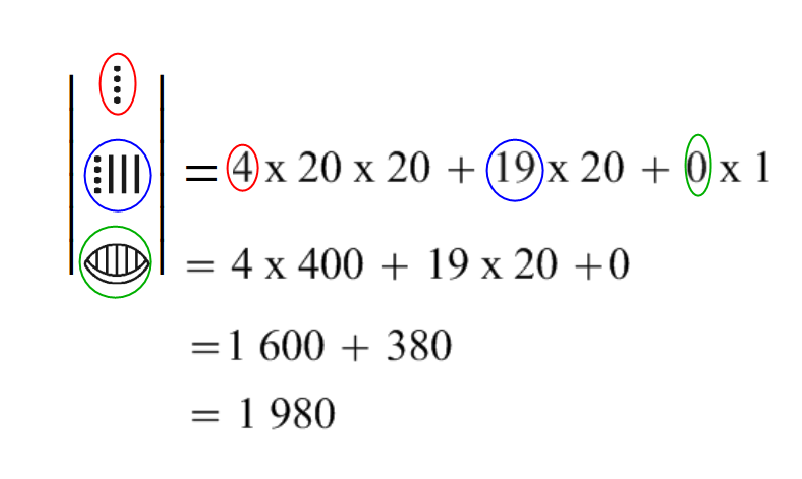
\includegraphics[scale=0.7]{maya7.eps} 
 \end{center}

Quel est   ce nombre ?\\


\includegraphics[scale=0.8]{maya1.eps} \\


\exo \\ Numération Maya\\

Pour les nombres plus grands que 19, les Mayas écrivaient les nombres sur plusieurs étages (de bas en haut), utilisant les puissances de 20. Un exemple :\\

 \begin{center}
 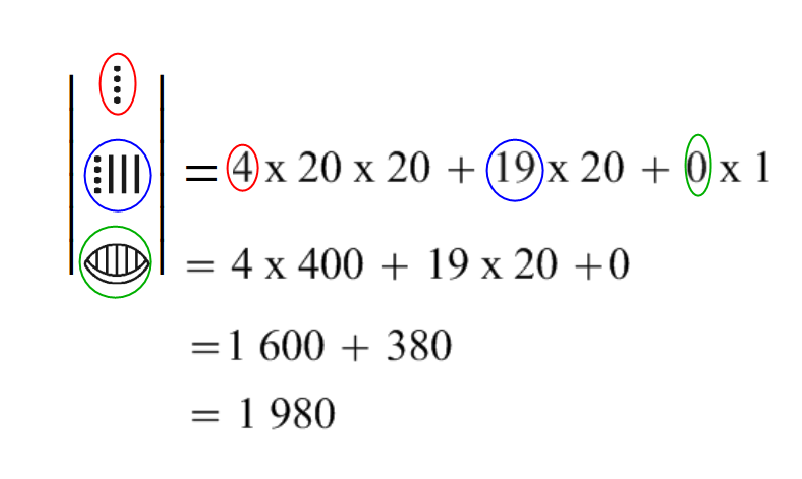
\includegraphics[scale=0.7]{maya7.eps} 
 \end{center}

Quel est   ce nombre ?\\


\includegraphics[scale=0.8]{maya2.eps} \\


\exo \\ Numération Maya\\

Pour les nombres plus grands que 19, les Mayas écrivaient les nombres sur plusieurs étages (de bas en haut), utilisant les puissances de 20. Un exemple :\\

 \begin{center}
 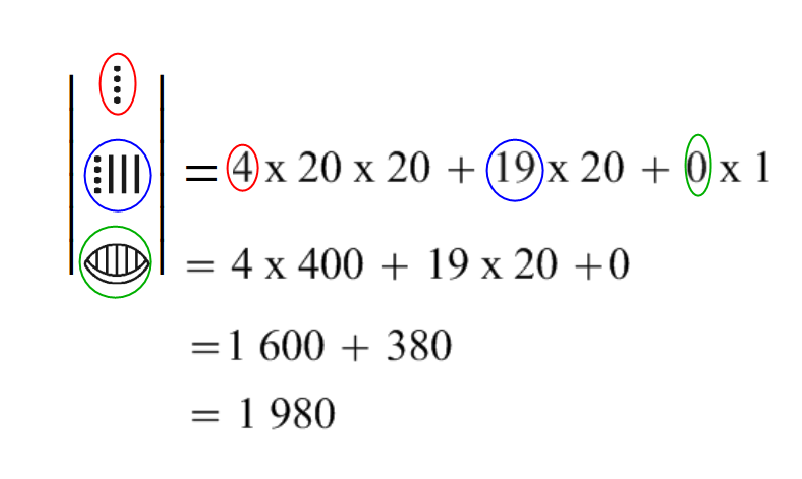
\includegraphics[scale=0.7]{maya7.eps} 
 \end{center}

Quel est   ce nombre ?\\


\includegraphics[scale=0.8]{maya3.eps} \\




\end{document}
